% Visão computacional do FRET: das imagens das câmeras à pose de preensão.
%
% Compilação (a partir desta pasta):
%   python3 ../../../scripts/vision_algorithm_figures.py   # figuras + dados.tex
%   latexmk -pdf algoritmo_visao.tex
\documentclass[11pt,a4paper]{article}

\usepackage[T1]{fontenc}
\usepackage[utf8]{inputenc}
\usepackage[brazil]{babel}
\usepackage{lmodern}
\usepackage{microtype}
\usepackage[margin=2.4cm]{geometry}
\usepackage{amsmath,amssymb,amsthm,mathtools,bm}
\usepackage{graphicx}
\usepackage{booktabs}
\usepackage{tabularx}
\usepackage{array}
\usepackage{float}
\usepackage[section]{placeins}
\usepackage[font=small,labelfont=bf]{caption}
\usepackage{subcaption}
\usepackage{xcolor}
\usepackage{tikz}
\usetikzlibrary{arrows.meta,positioning,shapes.geometric,calc}
\usepackage[
  locale=FR,
  output-decimal-marker={,},
  group-separator={.},
  group-minimum-digits=5,
  group-digits=integer,
  detect-all
]{siunitx}
\usepackage[colorlinks=true,linkcolor=blue!50!black,citecolor=green!40!black,urlcolor=blue!60!black]{hyperref}

% Gerado por scripts/vision_algorithm_figures.py -- nao editar.
\newcommand{\CircCircRf}{0.884}
\newcommand{\CircCircRba}{0.892}
\newcommand{\CircCircRda}{0.898}
\newcommand{\CircCircRga}{0.898}
\newcommand{\CircMecErrAboveHalfMax}{0.094}
\newcommand{\BiasOmxBiasMaxPx}{0.573}
\newcommand{\BiasOmxAlphaMaxDeg}{38.1}
\newcommand{\BiasOmxCheckMaxdiffPx}{0.000}
\newcommand{\BiasOmyBiasMaxPx}{1.390}
\newcommand{\BiasOmyAlphaMaxDeg}{40.2}
\newcommand{\BiasOmyCheckMaxdiffPx}{0.000}
\newcommand{\OmxCalOrth}{9.5e-11}
\newcommand{\OmxCalDet}{4.3e-11}
\newcommand{\OmxCalExt}{4.4e-11}
\newcommand{\OmxCalFx}{1.0e-08}
\newcommand{\OmxFx}{937.8321}
\newcommand{\OmxFovy}{42}
\newcommand{\OmxBallr}{20}
\newcommand{\OmxHsvBallFracInside}{100.00}
\newcommand{\OmxHsvBgFracInside}{0.00}
\newcommand{\OmxHsvBallHMedian}{34}
\newcommand{\OmxHsvBallSMedian}{196}
\newcommand{\OmxHsvBallVMedian}{231}
\newcommand{\OmxHsvBallHPab}{30}
\newcommand{\OmxHsvBallHPjj}{36}
\newcommand{\OmxHsvBallVPab}{130}
\newcommand{\OmxEU}{722.37}
\newcommand{\OmxEV}{327.41}
\newcommand{\OmxEUGt}{722.34}
\newcommand{\OmxEVGt}{327.45}
\newcommand{\OmxERadiusPx}{20.88}
\newcommand{\OmxEAreaPx}{1305.0}
\newcommand{\OmxEPerimeterPx}{135.88}
\newcommand{\OmxECirc}{0.8882}
\newcommand{\OmxET}{0.9059}
\newcommand{\OmxEWeight}{0.4961}
\newcommand{\OmxECentreErrPx}{0.05}
\newcommand{\OmxEIou}{0.984}
\newcommand{\OmxEDepth}{0.9059}
\newcommand{\OmxETanIncidence}{0.889}
\newcommand{\OmxENContours}{1}
\newcommand{\OmxEDcX}{0.08836}
\newcommand{\OmxEDwX}{0.37532}
\newcommand{\OmxEOX}{-0.120}
\newcommand{\OmxEPX}{220.01}
\newcommand{\OmxEDcY}{-0.03421}
\newcommand{\OmxEDwY}{-0.55199}
\newcommand{\OmxEOY}{0.300}
\newcommand{\OmxEPY}{-200.06}
\newcommand{\OmxEDcZ}{1.00000}
\newcommand{\OmxEDwZ}{-0.75062}
\newcommand{\OmxEOZ}{0.700}
\newcommand{\OmxEPZ}{20.00}
\newcommand{\OmxEEllA}{20.80}
\newcommand{\OmxEEllB}{20.71}
\newcommand{\OmxEEllBias}{0.043}
\newcommand{\OmxEEllAlpha}{5.41}
\newcommand{\OmxEEllDist}{0.9099}
\newcommand{\OmxEEllArea}{1353.5}
\newcommand{\OmxESegpx}{1342}
\newcommand{\OmxEJAa}{-0.7199}
\newcommand{\OmxEJAb}{-0.8043}
\newcommand{\OmxEJBa}{-0.6441}
\newcommand{\OmxEJBb}{1.0072}
\newcommand{\OmxEJsig}{1.291}
\newcommand{\OmxDU}{764.56}
\newcommand{\OmxDV}{468.25}
\newcommand{\OmxDUGt}{764.63}
\newcommand{\OmxDVGt}{468.04}
\newcommand{\OmxDRadiusPx}{25.21}
\newcommand{\OmxDAreaPx}{1898.5}
\newcommand{\OmxDPerimeterPx}{162.61}
\newcommand{\OmxDCirc}{0.9022}
\newcommand{\OmxDT}{0.7550}
\newcommand{\OmxDWeight}{0.5039}
\newcommand{\OmxDCentreErrPx}{0.22}
\newcommand{\OmxDIou}{0.988}
\newcommand{\OmxDDepth}{0.7551}
\newcommand{\OmxDTanIncidence}{0.521}
\newcommand{\OmxDNContours}{1}
\newcommand{\OmxDDcX}{0.13335}
\newcommand{\OmxDDwX}{0.45006}
\newcommand{\OmxDOX}{-0.120}
\newcommand{\OmxDPX}{219.80}
\newcommand{\OmxDDcY}{0.11596}
\newcommand{\OmxDDwY}{0.13238}
\newcommand{\OmxDOY}{-0.300}
\newcommand{\OmxDPY}{-200.05}
\newcommand{\OmxDDcZ}{1.00000}
\newcommand{\OmxDDwZ}{-0.90064}
\newcommand{\OmxDOZ}{0.700}
\newcommand{\OmxDPZ}{20.00}
\newcommand{\OmxDEllA}{25.23}
\newcommand{\OmxDEllB}{24.85}
\newcommand{\OmxDEllBias}{0.116}
\newcommand{\OmxDEllAlpha}{10.02}
\newcommand{\OmxDEllDist}{0.7668}
\newcommand{\OmxDEllArea}{1969.7}
\newcommand{\OmxDSegpx}{1946}
\newcommand{\OmxDJAa}{0.4374}
\newcommand{\OmxDJAb}{-0.7859}
\newcommand{\OmxDJBa}{-0.6759}
\newcommand{\OmxDJBb}{-0.4309}
\newcommand{\OmxDJsig}{0.905}
\newcommand{\OmxGtX}{220.00}
\newcommand{\OmxFuX}{219.91}
\newcommand{\OmxGtY}{-200.00}
\newcommand{\OmxFuY}{-200.05}
\newcommand{\OmxGtZ}{20.00}
\newcommand{\OmxFuZ}{20.00}
\newcommand{\OmxExXyerr}{0.108}
\newcommand{\OmxExZerr}{0.000}
\newcommand{\OmxJacFd}{3.8e-13}
\newcommand{\OmxMcEmpMinMm}{0.329}
\newcommand{\OmxMcEmpMaxMm}{0.382}
\newcommand{\OmxMcPredMinMm}{0.327}
\newcommand{\OmxMcPredMaxMm}{0.380}
\newcommand{\OmxMcFrobRel}{0.010}
\newcommand{\OmxDzShift}{0.578}
\newcommand{\OmxIkHoverMm}{0.004}
\newcommand{\OmxIkGraspMm}{0.000}
\newcommand{\OmxIkLiftMm}{0.003}
\newcommand{\OccVisibleFrac}{12.1}
\newcommand{\OccCentreErrPx}{16.28}
\newcommand{\OccCirc}{0.51}
\newcommand{\OccRadiusPx}{13.73}
\newcommand{\OccAPx}{22.38}
\newcommand{\occMonoErr}{0.14}
\newcommand{\occLeftErr}{17.61}
\newcommand{\occLeftW}{0.363}
\newcommand{\occFusedErr}{6.40}
\newcommand{\OmxMecGap}{1.0e-04}
\newcommand{\OmxSwN}{9}
\newcommand{\OmxSwDet}{9}
\newcommand{\OmxSwMedian}{0.14}
\newcommand{\OmxSwMax}{6.40}
\newcommand{\OmxGridN}{208}
\newcommand{\OmxGridDet}{208}
\newcommand{\OmxGridDual}{165}
\newcommand{\OmxGridMedian}{0.25}
\newcommand{\OmxGridPjf}{7.49}
\newcommand{\OmxGridMax}{17.20}
\newcommand{\OmxGridClearN}{93}
\newcommand{\OmxGridClearMax}{0.73}
\newcommand{\OmxGridClearMedian}{0.14}
\newcommand{\OmyCalOrth}{1.3e-10}
\newcommand{\OmyCalDet}{7.6e-11}
\newcommand{\OmyCalExt}{4.9e-11}
\newcommand{\OmyCalFx}{4.6e-08}
\newcommand{\OmyFx}{869.1169}
\newcommand{\OmyFovy}{45}
\newcommand{\OmyBallr}{43}
\newcommand{\OmyHsvBallFracInside}{99.98}
\newcommand{\OmyHsvBgFracInside}{0.01}
\newcommand{\OmyHsvBallHMedian}{34}
\newcommand{\OmyHsvBallSMedian}{196}
\newcommand{\OmyHsvBallVMedian}{230}
\newcommand{\OmyHsvBallHPab}{30}
\newcommand{\OmyHsvBallHPjj}{36}
\newcommand{\OmyHsvBallVPab}{125}
\newcommand{\OmyEU}{752.67}
\newcommand{\OmyEV}{326.21}
\newcommand{\OmyEUGt}{752.58}
\newcommand{\OmyEVGt}{326.46}
\newcommand{\OmyERadiusPx}{29.46}
\newcommand{\OmyEAreaPx}{2609.0}
\newcommand{\OmyEPerimeterPx}{191.34}
\newcommand{\OmyECirc}{0.8955}
\newcommand{\OmyET}{1.2837}
\newcommand{\OmyEWeight}{0.5015}
\newcommand{\OmyECentreErrPx}{0.27}
\newcommand{\OmyEIou}{0.991}
\newcommand{\OmyEDepth}{1.2834}
\newcommand{\OmyETanIncidence}{0.955}
\newcommand{\OmyENContours}{1}
\newcommand{\OmyEDcX}{0.13021}
\newcommand{\OmyEDwX}{0.41307}
\newcommand{\OmyEOX}{-0.180}
\newcommand{\OmyEPX}{350.26}
\newcommand{\OmyEDcY}{-0.03831}
\newcommand{\OmyEDwY}{-0.56126}
\newcommand{\OmyEOY}{0.420}
\newcommand{\OmyEPY}{-300.48}
\newcommand{\OmyEDcZ}{1.00000}
\newcommand{\OmyEDwZ}{-0.72992}
\newcommand{\OmyEOZ}{0.980}
\newcommand{\OmyEPZ}{43.00}
\newcommand{\OmyEEllA}{29.40}
\newcommand{\OmyEEllB}{29.14}
\newcommand{\OmyEEllBias}{0.132}
\newcommand{\OmyEEllAlpha}{7.72}
\newcommand{\OmyEEllDist}{1.2951}
\newcommand{\OmyEEllArea}{2691.5}
\newcommand{\OmyESegpx}{2668}
\newcommand{\OmyEJAa}{-1.0050}
\newcommand{\OmyEJAb}{-1.3653}
\newcommand{\OmyEJBa}{-1.0823}
\newcommand{\OmyEJBb}{1.5035}
\newcommand{\OmyEJsig}{2.039}
\newcommand{\OmyDU}{769.25}
\newcommand{\OmyDV}{470.18}
\newcommand{\OmyDUGt}{769.31}
\newcommand{\OmyDVGt}{469.67}
\newcommand{\OmyDRadiusPx}{35.82}
\newcommand{\OmyDAreaPx}{3851.0}
\newcommand{\OmyDPerimeterPx}{233.14}
\newcommand{\OmyDCirc}{0.8903}
\newcommand{\OmyDT}{1.0625}
\newcommand{\OmyDWeight}{0.4985}
\newcommand{\OmyDCentreErrPx}{0.52}
\newcommand{\OmyDIou}{0.991}
\newcommand{\OmyDDepth}{1.0630}
\newcommand{\OmyDTanIncidence}{0.579}
\newcommand{\OmyDNContours}{1}
\newcommand{\OmyDDcX}{0.14929}
\newcommand{\OmyDDwX}{0.49815}
\newcommand{\OmyDOX}{-0.180}
\newcommand{\OmyDPX}{349.31}
\newcommand{\OmyDDcY}{0.12735}
\newcommand{\OmyDDwY}{0.11272}
\newcommand{\OmyDOY}{-0.420}
\newcommand{\OmyDPY}{-300.23}
\newcommand{\OmyDDcZ}{1.00000}
\newcommand{\OmyDDwZ}{-0.88184}
\newcommand{\OmyDOZ}{0.980}
\newcommand{\OmyDPZ}{43.00}
\newcommand{\OmyDEllA}{35.86}
\newcommand{\OmyDEllB}{35.19}
\newcommand{\OmyDEllBias}{0.279}
\newcommand{\OmyDEllAlpha}{11.08}
\newcommand{\OmyDEllDist}{1.0832}
\newcommand{\OmyDEllArea}{3963.7}
\newcommand{\OmyDSegpx}{3919}
\newcommand{\OmyDJAa}{0.6066}
\newcommand{\OmyDJAb}{-1.2644}
\newcommand{\OmyDJBa}{-1.0615}
\newcommand{\OmyDJBb}{-0.5816}
\newcommand{\OmyDJsig}{1.408}
\newcommand{\OmyGtX}{350.00}
\newcommand{\OmyFuX}{349.79}
\newcommand{\OmyGtY}{-300.00}
\newcommand{\OmyFuY}{-300.36}
\newcommand{\OmyGtZ}{43.00}
\newcommand{\OmyFuZ}{43.00}
\newcommand{\OmyExXyerr}{0.418}
\newcommand{\OmyExZerr}{0.000}
\newcommand{\OmyJacFd}{7.1e-13}
\newcommand{\OmyMcEmpMinMm}{0.502}
\newcommand{\OmyMcEmpMaxMm}{0.603}
\newcommand{\OmyMcPredMinMm}{0.500}
\newcommand{\OmyMcPredMaxMm}{0.600}
\newcommand{\OmyMcFrobRel}{0.011}
\newcommand{\OmyDzShift}{0.651}
\newcommand{\OmyIkHoverMm}{0.000}
\newcommand{\OmyIkGraspMm}{0.001}
\newcommand{\OmyIkLiftMm}{0.000}
\newcommand{\OmyMecGap}{1.0e-04}
\newcommand{\OmySwN}{9}
\newcommand{\OmySwDet}{8}
\newcommand{\OmySwMedian}{0.50}
\newcommand{\OmySwMax}{3.69}
\newcommand{\OmyGridN}{210}
\newcommand{\OmyGridDet}{199}
\newcommand{\OmyGridDual}{100}
\newcommand{\OmyGridMedian}{0.75}
\newcommand{\OmyGridPjf}{30.37}
\newcommand{\OmyGridMax}{37.97}
\newcommand{\OmyGridClearN}{38}
\newcommand{\OmyGridClearMax}{0.70}
\newcommand{\OmyGridClearMedian}{0.43}

\makeatletter
\newcommand{\tabelagerada}[1]{\@@input #1 }
\makeatother

\setlength{\emergencystretch}{3em}

\newtheorem{proposicao}{Proposição}
\newtheorem{lema}[proposicao]{Lema}
\newtheorem{corolario}[proposicao]{Corolário}
\theoremstyle{definition}
\newtheorem{definicao}{Definição}
\theoremstyle{remark}
\newtheorem{observacao}{Observação}

\newcommand{\R}{\mathbb{R}}
\newcommand{\Z}{\mathbb{Z}}
\newcommand{\T}{^{\mkern-1.5mu\mathsf{T}}}
\newcommand{\vect}[1]{\bm{#1}}
\newcommand{\ez}{\vect{e}_z}
\newcommand{\code}[1]{\texttt{\detokenize{#1}}}
\DeclareMathOperator{\HSV}{hsv}
\DeclareMathOperator{\MEC}{MEC}
\DeclareMathOperator*{\argmax}{arg\,max}
\DeclareMathOperator*{\argmin}{arg\,min}

\title{\textbf{Visão computacional para \emph{pick-and-place} no FRET}\\[2pt]
\large Das imagens das câmeras à pose de preensão da bola:\\
modelo matemático, implementação e análise de erro}
\author{FRET --- módulo \texttt{fret.vision}}
\date{Outubro de 2026}

\begin{document}
\maketitle

\begin{abstract}
\noindent
Este documento descreve, com rigor matemático, o algoritmo de visão que o FRET
usa para localizar uma bola sobre a mesa e transformar essa localização em
alvos de preensão para os manipuladores OpenMANIPULATOR-X (OM-X) e
OpenMANIPULATOR-Y (OMY). A cadeia completa é: renderização de duas câmeras
calibradas no MuJoCo; segmentação por limiar no espaço HSV; filtragem
morfológica; extração de contornos e seleção pela circularidade; estimação do
centro pelo círculo envolvente mínimo; retroprojeção do pixel como um raio no
mundo; interseção com o plano horizontal que contém o centro da bola; fusão
das vistas por média ponderada; e cinemática inversa do ponto médio dos dedos
da garra. Para cada etapa apresentamos a formulação, as hipóteses e
proposições com demonstração (forma da silhueta da esfera projetada, viés de
perspectiva, comportamento do círculo envolvente mínimo sob oclusão, limite
digital da circularidade, jacobiano da elevação ao plano). Todos os números
foram produzidos executando o código do repositório
(\code{scripts/vision_algorithm_figures.py}), e as fórmulas fechadas foram
verificadas numericamente contra a implementação.
\end{abstract}

\tableofcontents
\newpage

%=====================================================================
\section{Visão geral}
\label{sec:visao-geral}
%=====================================================================

O problema resolvido pelo módulo \code{fret.vision} é o seguinte: dado um
conjunto de imagens RGB de $N \geq 1$ câmeras com calibração conhecida, estimar
a posição $\vect{p}^\star\in\R^3$, no referencial do mundo, do centro de uma bola
de raio conhecido $r$ apoiada sobre uma mesa horizontal de altura conhecida
$z_{\text{mesa}}$. A posição estimada $\hat{\vect p}$ é então usada pelo
controlador para calcular as configurações articulares de aproximação,
preensão e elevação.

A Figura~\ref{fig:pipeline} resume o fluxo. O código está organizado em três
estágios atrás de protocolos independentes do algoritmo
(\code{fret/vision/protocols.py}): um \emph{detector} (imagem $\to$ hipóteses
em pixels), um \emph{rastreador} opcional (não usado na configuração atual) e
um \emph{elevador de pose} (pixels $\to$ mundo). A orquestração está em
\code{BallVisionPipeline.process} (\code{fret/vision/pipeline.py}), e a
montagem concreta, em \code{fret/vision/factory.py}.

\begin{figure}[ht]
\centering
\begin{tikzpicture}[
  node distance=4mm and 5mm,
  blk/.style={draw, rounded corners=2pt, fill=#1, align=center,
              font=\footnotesize, minimum height=10mm, text width=27mm},
  blk/.default={blue!6},
  lab/.style={font=\scriptsize\itshape, text=black!65},
  >={Stealth[length=2mm]}
]
\node[blk=gray!10] (cam) {Câmeras MuJoCo\\ esquerda e direita\\ $1280\times720$};
\node[blk, right=of cam] (hsv) {RGB $\to$ HSV\\ limiar $[\vect\ell,\vect h]$\\ (Sec.~\ref{sec:segmentacao})};
\node[blk, right=of hsv] (morph) {Abertura e\\ fechamento\\ (Sec.~\ref{sec:morfologia})};
\node[blk, right=of morph] (cont) {Contornos,\\ circularidade,\\ MEC (Sec.~\ref{sec:contornos})};
\node[blk=green!8, below=9mm of cont] (lift) {Raio $\cap$ plano\\ $z=z_{\text{mesa}}+r$\\ (Sec.~\ref{sec:elevacao})};
\node[blk=green!8, left=of lift] (fuse) {Fusão ponderada\\ das vistas\\ (Sec.~\ref{sec:fusao})};
\node[blk=orange!10, left=of fuse] (obs) {{\scriptsize\code{BallObservation}}\\ $\hat{\vect p}\in\R^3$};
\node[blk=orange!10, left=of obs] (ik) {Alvos de preensão\\ + IK dos dedos\\ (Sec.~\ref{sec:preensao})};
\draw[->] (cam) -- node[lab, above]{$I$} (hsv);
\draw[->] (hsv) -- node[lab, above]{$M_0$} (morph);
\draw[->] (morph) -- node[lab, above]{$M$} (cont);
\draw[->] (cont) -- node[lab, right]{$(\hat u,\hat v),\,c$} (lift);
\draw[->] (lift) -- node[lab, above]{$\hat{\vect p}_i$} (fuse);
\draw[->] (fuse) -- (obs);
\draw[->] (obs) -- (ik);
\node[lab, above=1mm of cam, xshift=0mm] {\code{fret.simulation}};
\node[lab, above=1mm of morph, xshift=0mm] {\code{HsvBlobBallDetector}};
\node[lab, below=1mm of fuse] {\code{TablePlanePoseLifter}};
\node[lab, below=1mm of ik] {\code{fret.control.pick_place_vision}};
\end{tikzpicture}
\caption{Fluxo completo, das imagens à preensão. Azul: detector em espaço de
imagem; verde: geometria no mundo; laranja: consumidores no controle. Cada
vista é processada de forma independente até a fusão.}
\label{fig:pipeline}
\end{figure}

\paragraph{Cenário.} Nas células de \emph{pick-and-place} (OM-X e OMY), duas
câmeras ficam presas nos cantos superiores de um pórtico estrutural atrás do
braço (\code{docs/vision/camera-layout.md}). A bola é amarelo-esverdeada (cor
do material $\text{RGBA}=(0{,}85;\,0{,}92;\,0{,}20;\,1)$) e tem raio
\SI{\OmxBallr}{mm} na célula OM-X e \SI{\OmyBallr}{mm} na célula OMY. A
Figura~\ref{fig:cameras} mostra as duas vistas na pose de coleta padrão do
OM-X, e a Figura~\ref{fig:overview}, a estimativa final sobreposta à cena.

\begin{figure}[ht]
\centering
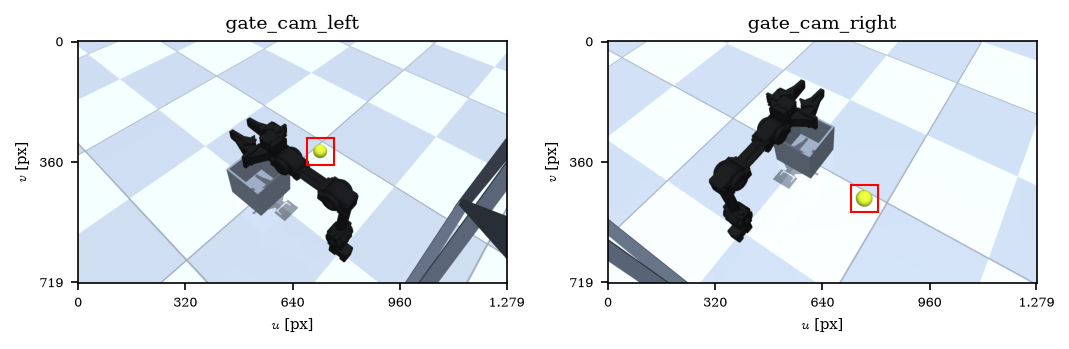
\includegraphics[width=\linewidth]{figuras/cameras_omx.png}
\caption{Imagens reais renderizadas pelas duas câmeras do pórtico (OM-X, bola em
$(0{,}22;\,-0{,}20)$\,m). O quadrado vermelho marca a região da bola ampliada na
Figura~\ref{fig:mascara}.}
\label{fig:cameras}
\end{figure}

\begin{figure}[ht]
\centering
\begin{subfigure}{0.49\linewidth}
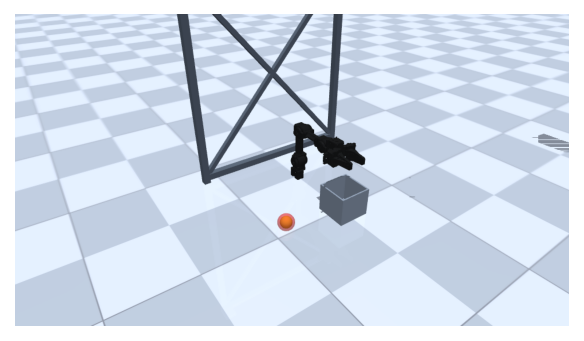
\includegraphics[width=\linewidth]{figuras/overview_omx.png}
\caption{OM-X}
\end{subfigure}\hfill
\begin{subfigure}{0.49\linewidth}
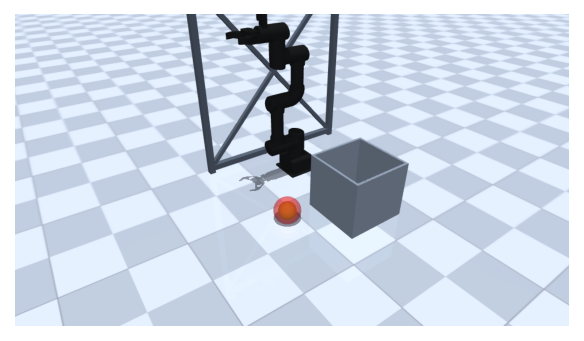
\includegraphics[width=\linewidth]{figuras/overview_omy.png}
\caption{OMY}
\end{subfigure}
\caption{Vista geral das células. A esfera vermelha translúcida
(\code{cv_ball_ghost}, apenas visual) é posicionada na estimativa de visão
$\hat{\vect p}$; a bola amarela real fica dentro dela.}
\label{fig:overview}
\end{figure}

\paragraph{Notação.} Vetores em negrito; $\ez=(0,0,1)\T$; $\tilde{\vect u} =
(u,v,1)\T$ são coordenadas homogêneas de pixel; $[\,\cdot\,]_{xy}$ é a
projeção nas duas primeiras componentes. Ângulos em radianos, salvo
indicação. Os índices $E$ e $D$ referem-se às câmeras esquerda
(\code{gate_cam_left}) e direita (\code{gate_cam_right}).

%=====================================================================
\section{Modelo de câmera}
\label{sec:camera}
%=====================================================================

\subsection{Referenciais}

Usamos três referenciais: o mundo $\{W\}$ (origem na base do braço, $x$ para
frente, $z$ para cima); a câmera do MuJoCo $\{M\}$, que olha ao longo de $-z_M$
com $y_M$ para cima na imagem; e a câmera óptica no padrão do OpenCV $\{C\}$, com
$x_C$ para a direita, $y_C$ para baixo e $z_C$ para dentro da cena. Todo o
pipeline trabalha em $\{C\}$.

O MuJoCo fornece a posição $\vect O\in\R^3$ do centro óptico (\code{cam_xpos}) e
a matriz $R_M\in SO(3)$ (\code{cam_xmat}), cujas colunas são os eixos de $\{M\}$
expressos em $\{W\}$. Como $x_C=x_M$, $y_C=-y_M$ e $z_C=-z_M$, temos
\begin{equation}
R \;=\; R_M\,\operatorname{diag}(1,-1,-1),
\qquad
T_{WC} = \begin{bmatrix} R & \vect O\\ \vect 0\T & 1\end{bmatrix},
\label{eq:mj2cv}
\end{equation}
implementado em \code{mujoco_xmat_to_opencv_rotation}
(\code{fret/simulation/mujoco_camera.py}). $R$ continua sendo uma rotação:
é produto de matrizes ortogonais e $\det R = \det R_M \cdot (1)(-1)(-1) = 1$.
A transformação leva coordenadas da câmera para o mundo:
$\vect x_W = R\,\vect x_C + \vect O$.

\subsection{Projeção \emph{pinhole} e intrínsecos}

Com a matriz de intrínsecos
\begin{equation}
K=\begin{bmatrix} f_x & 0 & c_x\\ 0 & f_y & c_y\\ 0&0&1\end{bmatrix},
\end{equation}
um ponto $\vect x_W$ à frente da câmera é projetado em
\begin{equation}
\vect x_C = R\T(\vect x_W-\vect O)=(X,Y,Z)\T,\qquad
u = f_x\frac{X}{Z}+c_x,\quad v=f_y\frac{Y}{Z}+c_y,\quad Z>0.
\label{eq:proj}
\end{equation}
O simulador não tem distorção de lente, e o tipo \code{CameraIntrinsics}
deliberadamente omite coeficientes de distorção.

O MuJoCo define a câmera pelo campo de visão vertical $\phi_y$ (\code{fovy}).
No plano $Z=1$, a meia-altura visível é $\tan(\phi_y/2)$ e corresponde a $H/2$
pixels; com pixels quadrados,
\begin{equation}
f_x=f_y=f=\frac{H/2}{\tan(\phi_y/2)},\qquad
c_x=\frac{W-1}{2},\quad c_y=\frac{H-1}{2},
\label{eq:fovy}
\end{equation}
(\code{intrinsics_from_fovy}). O ponto principal usa a convenção de que o pixel
de índice $(i,j)$ tem centro nas coordenadas inteiras $(i,j)$, a mesma do
OpenCV para contornos. Para $H=720$: com $\phi_y=\ang{\OmxFovy}$ (OM-X),
$f=360/\tan(\ang{21})=\num{\OmxFx}$\,px; com $\phi_y=\ang{\OmyFovy}$ (OMY),
$f=360/\tan(\ang{22.5})=\num{\OmyFx}$\,px. Em ambos os casos,
$(c_x,c_y)=(\num{639.5}; \num{359.5})$.

\paragraph{Consistência da calibração.} As matrizes $K$ e
$T_{WC}$ de cada câmera ficam guardadas nos arquivos de configuração
\code{omx_portal_overhead.yml} e \code{omy_portal_overhead.yml}. Verificamos contra o modelo MuJoCo carregado:
a maior diferença entre os $T_{WC}$ do YAML e os calculados a partir do modelo
foi \num{\OmxCalExt} (OM-X) e \num{\OmyCalExt} (OMY); a diferença em $f$ e
$c$ foi $\leq\num{\OmyCalFx}$\,px; e
$\max|R\T R-I|\leq\num{\OmyCalOrth}$, com $|\det R-1|\leq\num{\OmyCalDet}$.
Portanto, a calibração usada pelo pipeline coincide com a geometria
renderizada até o arredondamento do YAML.

%=====================================================================
\section{Segmentação por cor no espaço HSV}
\label{sec:segmentacao}
%=====================================================================

\subsection{\texorpdfstring{Conversão RGB $\to$ HSV (OpenCV, 8 bits)}{Conversão RGB para HSV (OpenCV, 8 bits)}}

Seja $I:\Omega\to\{0,\dots,255\}^3$ a imagem RGB, com
$\Omega=\{0,\dots,W-1\}\times\{0,\dots,H-1\}$. Para um pixel $(R,G,B)$, sejam
$M_{\max}=\max(R,G,B)$, $m=\min(R,G,B)$ e $\Delta=M_{\max}-m$. O OpenCV calcula
\begin{align}
V &= M_{\max},\qquad
S = \begin{cases} 255\,\Delta/M_{\max}, & M_{\max}>0\\ 0,& M_{\max}=0\end{cases}\\
H' &= \begin{cases}
60\,(G-B)/\Delta, & M_{\max}=R\\
120+60\,(B-R)/\Delta, & M_{\max}=G\\
240+60\,(R-G)/\Delta, & M_{\max}=B
\end{cases}\quad (H'\leftarrow H'+360 \text{ se } H'<0),
\qquad H = H'/2,
\end{align}
com arredondamento para inteiro. Assim $H\in\{0,\dots,179\}$ representa o
matiz em graus divididos por dois, e $S,V\in\{0,\dots,255\}$. O código
converte RGB$\to$BGR$\to$HSV (\code{_to_bgr} e \code{cv2.cvtColor}).

\paragraph{Exemplo.} A cor difusa do material da bola,
$(217;\,235;\,51)$, tem $M_{\max}=G=235$, $m=51$ e $\Delta=184$. Logo $V=235$,
$S=255\cdot184/235\approx199{,}7\to200$ e
$H'=120+60(51-217)/184\approx65{,}9$, ou seja, $H=33$. A chamada
\code{cv2.cvtColor} retorna exatamente $(33;\,200;\,235)$.

\subsection{Limiar}

\begin{definicao}[Máscara de cor]
Dados limites $\vect\ell,\vect h\in\{0,\dots,255\}^3$, a máscara inicial é
\begin{equation}
M_0(\vect x) = \begin{cases}255, & \vect\ell\preceq \HSV(I(\vect x))\preceq\vect h\\ 0,&\text{caso contrário,}\end{cases}
\end{equation}
em que $\preceq$ é a ordem componente a componente, com limites inclusivos
(\code{cv2.inRange}). Se a configuração define um segundo intervalo
$[\vect\ell',\vect h']$, usa-se $M_0\leftarrow M_0\vee M_0'$. Isso existe porque o
matiz é circular: um objeto vermelho ocupa $H\approx 0$ e $H\approx179$ e
precisa de dois intervalos.
\end{definicao}

Nas células com pórtico, $\vect\ell=(20;\,40;\,40)$ e $\vect h=(50;\,255;\,255)$, sem
segundo intervalo. A Figura~\ref{fig:hsv} justifica a escolha com dados: os
pixels da bola, identificados pela renderização de segmentação do MuJoCo (a
verdade de campo), concentram-se em $H\in[\num{\OmxHsvBallHPab}; \num{\OmxHsvBallHPjj}]$
(percentis 1 e 99), com mediana $(H,S,V)=(\num{\OmxHsvBallHMedian}; \num{\OmxHsvBallSMedian}; \num{\OmxHsvBallVMedian})$. O piso e o pórtico ficam em
$H\approx 90$--$120$ ou têm $S$ baixo. Na vista da pose padrão,
\SI{\OmxHsvBallFracInside}{\percent} dos pixels da bola caem dentro da caixa de
limiar e \SI{\OmxHsvBgFracInside}{\percent} de uma amostra de \num{80000}
pixels de fundo caem dentro dela (OMY: \SI{\OmyHsvBallFracInside}{\percent} e
\SI{\OmyHsvBgFracInside}{\percent}). O valor $V$ mínimo da bola
(\num{\OmxHsvBallVPab}, no lado sombreado) está bem acima de $\ell_V=40$, o que
dá margem para variação de iluminação.

\begin{figure}[ht]
\centering
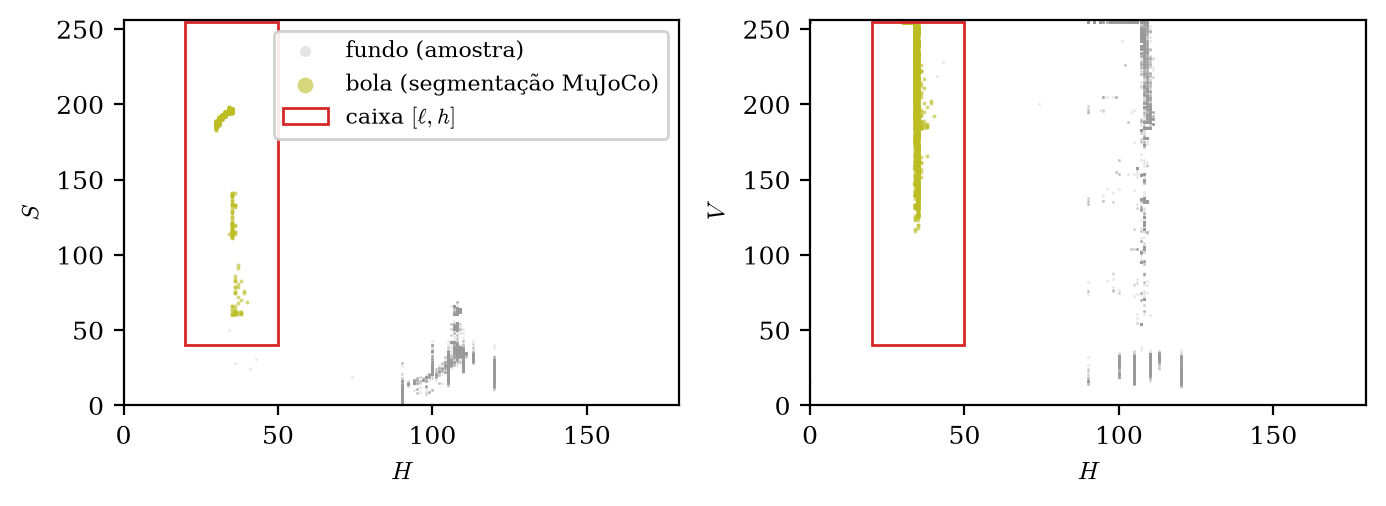
\includegraphics[width=0.92\linewidth]{figuras/hsv_omx.png}
\caption{Distribuição dos pixels da bola (verde-oliva, rótulos da
segmentação do MuJoCo) e de uma amostra do fundo (cinza) nos planos $H$--$S$ e
$H$--$V$, com a caixa de limiar $[\vect\ell,\vect h]$ da configuração OM-X.
As duas câmeras estão incluídas.}
\label{fig:hsv}
\end{figure}

%=====================================================================
\section{Filtragem morfológica}
\label{sec:morfologia}
%=====================================================================

Identificamos a máscara binária com o conjunto $X=\{\vect x\in\Omega:
M_0(\vect x)\neq0\}\subset\Z^2$. Seja $B\subset\Z^2$ um elemento estruturante
simétrico ($B=-B$) centrado na origem e $B_{\vect x}=\vect x+B$.

\begin{definicao}
Erosão $X\ominus B=\{\vect x: B_{\vect x}\subseteq X\}$; dilatação
$X\oplus B=\{\vect x: B_{\vect x}\cap X\neq\emptyset\}$; abertura
$X\circ B=(X\ominus B)\oplus B$; fechamento $X\bullet B=(X\oplus B)\ominus B$.
\end{definicao}

O detector aplica $M = (M_0\circ B)\bullet B$ (\code{mask_for_frame}), com
o elemento estruturante devolvido por
\[
\text{\code{cv2.getStructuringElement(cv2.MORPH_ELLIPSE, (5, 5))}}\,:
\]
\[
B=\begin{bmatrix}
0&0&1&0&0\\1&1&1&1&1\\1&1&1&1&1\\1&1&1&1&1\\0&0&1&0&0
\end{bmatrix}.
\]

\begin{proposicao}[Propriedades usadas]
\label{prop:morph}
(i) $X\circ B=\bigcup\{B_{\vect y}: B_{\vect y}\subseteq X\}\subseteq X$, ou seja,
a abertura mantém exatamente os pontos cobertos por alguma translação de $B$
contida em $X$. (ii) $X\subseteq X\bullet B$ e
$(X\bullet B)^c=X^c\circ B$. (iii) As duas operações são crescentes e
idempotentes.
\end{proposicao}
\begin{proof}
(i) $\vect z\in(X\ominus B)\oplus B$ se e só se existe $\vect y$ com
$B_{\vect y}\subseteq X$ e $\vect z\in B_{\vect y}$ (simetria de $B$). (ii) Pela
dualidade $(X\oplus B)^c=X^c\ominus B$, temos $(X\bullet B)^c=(X^c\ominus
B)\oplus B=X^c\circ B$; a inclusão segue de (i) aplicado a $X^c$. (iii) É o
resultado clássico de Matheron e Serra \cite{serra1982}.
\end{proof}

Consequência prática: pela Proposição~\ref{prop:morph}(i), a abertura apaga
qualquer componente de falso positivo que não contenha uma cópia de $B$
(pontos isolados, linhas de 1 a 2\,px de largura em bordas de objetos). Pelo
item (ii), o fechamento preenche furos e reentrâncias do complemento que não
contêm $B$, como o reflexo especular ou o recorte deixado por uma aresta fina
à frente da bola. Para a bola sem oclusão, de raio $\approx 20$--$36$\,px, as
duas operações quase não alteram a silhueta (Figura~\ref{fig:mascara}).

\begin{figure}[ht]
\centering
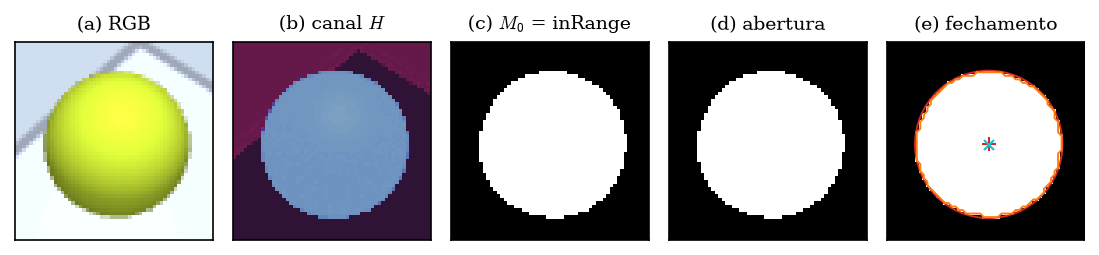
\includegraphics[width=\linewidth]{figuras/mascara_omx.png}
\caption{Etapas do detector na câmera esquerda (OM-X, pose padrão), recorte
de $56\times56$\,px. (e) Contorno externo (laranja), círculo envolvente mínimo
(vermelho) e centro estimado ($+$). O $\times$ ciano é a projeção exata do
centro da bola pela Eq.~\eqref{eq:proj}.}
\label{fig:mascara}
\end{figure}

%=====================================================================
\section{Contornos, circularidade e centro}
\label{sec:contornos}
%=====================================================================

\subsection{Extração de contornos}

O detector extrai as bordas externas das componentes 8-conexas de $M$ com o
algoritmo de seguimento de bordas de Suzuki e Abe \cite{suzuki1985}
(\code{cv2.findContours}, modo \code{RETR_EXTERNAL}). Cada contorno é um
polígono fechado $\mathcal P=(\vect q_0,\dots,\vect q_{n-1})$ cujos vértices são
centros de pixels de borda. O modo \code{CHAIN_APPROX_SIMPLE} só remove
vértices intermediários de trechos horizontais, verticais ou diagonais, de
modo que o polígono (como subconjunto do plano) não muda.

\subsection{Área, perímetro e circularidade}

\begin{equation}
A(\mathcal P)=\frac12\left|\sum_{k=0}^{n-1}\left(x_k y_{k+1}-x_{k+1}y_k\right)\right|,\qquad
P(\mathcal P)=\sum_{k=0}^{n-1}\|\vect q_{k+1}-\vect q_k\|,\qquad
c=\frac{4\pi A}{P^2},
\label{eq:circ}
\end{equation}
com índices módulo $n$ (\code{contourArea}, \code{arcLength},
\code{_circularity}). Como os vértices estão sobre a rede $\Z^2$, o teorema de
Pick dá, para um polígono simples, $A=I+B_\partial/2-1$, com $I$ pontos
interiores e $B_\partial$ pontos de rede na borda. Logo, $A$ fica cerca de meia
camada de pixels abaixo da contagem de pixels da componente. No exemplo da
Seção~\ref{sec:exemplo}, $A=\num{\OmxEAreaPx}$ contra
\num{\OmxESegpx} pixels visíveis da bola na segmentação de referência e
\num{\OmxEEllArea}\,px$^2$ de área teórica da silhueta.

Pela desigualdade isoperimétrica, $P^2\geq4\pi A$ para qualquer curva
plana fechada, com igualdade somente para o círculo. Portanto $c\in(0,1]$ e
$c=1$ caracteriza o disco no contínuo. No caso digital, o máximo atingível é
menor:

\begin{proposicao}[Limite digital da circularidade]
\label{prop:circ-digital}
Seja $\mathcal P_R$ o contorno externo de um disco digitalizado de raio $R$.
Quando $R\to\infty$,
\begin{equation}
\frac{P(\mathcal P_R)}{2\pi R}\;\to\;\frac{8}{\pi}(\sqrt2-1)\approx1{,}05479,
\qquad
c(\mathcal P_R)\;\to\;c_\infty=\Bigl(\frac{\pi}{8(\sqrt2-1)}\Bigr)^2\approx0{,}8988.
\end{equation}
\end{proposicao}
\begin{proof}
Por simetria, basta um octante. Nele, a tangente ao círculo faz ângulo
$\theta\in[0,\pi/4]$ com o eixo dominante, e o contorno é um caminho 8-conexo
de passos axiais (comprimento 1) e diagonais ($\sqrt2$). Por unidade de avanço
no eixo dominante, o caminho dá $\tan\theta$ passos diagonais e $1-\tan\theta$
passos axiais. Como um elemento de arco $ds$ avança $\cos\theta\,ds$, o
comprimento do caminho por unidade de arco é
$\cos\theta\,[(1-\tan\theta)+\sqrt2\tan\theta]=\cos\theta+(\sqrt2-1)\sin\theta$.
No círculo, $\theta$ é proporcional ao comprimento de arco; a média no
octante é
\[
\frac{4}{\pi}\int_0^{\pi/4}\bigl(\cos\theta+(\sqrt2-1)\sin\theta\bigr)\,d\theta
=\frac4\pi\bigl(2\sqrt2-2\bigr)=\frac{8}{\pi}(\sqrt2-1).
\]
O erro relativo de área é $O(P/R^2)=O(1/R)$, de modo que
$A/(\pi R^2)\to1$, e o limite de $c$ segue de \eqref{eq:circ}.
\end{proof}

A Figura~\ref{fig:circ}(a) confirma a proposição numericamente com o mesmo
código OpenCV: a circularidade média de discos digitais é \num{\CircCircRf} em
$R=5$\,px, \num{\CircCircRda} em $R=30$\,px e \num{\CircCircRga} em
$R=60$\,px, ou seja, $c_\infty$ com três casas. Isso explica por que o
limiar configurado, $c_{\min}=0{,}45$ (pórtico) ou $0{,}55$ (fixture), está
bem abaixo de 1. A silhueta de uma esfera é uma elipse levemente alongada
(Seção~\ref{sec:silhueta}). Mesmo no canto da imagem, com razão de eixos
$b/a\approx\cos\alpha\approx0{,}76$, a circularidade contínua dessa elipse é
$\approx0{,}97$, o que ainda deixa grande margem até $c_{\min}$.

\subsection{Filtros e seleção}

Um contorno é aceito se $A_{\min}\leq A\leq A_{\max}$ e $c\geq c_{\min}$. Entre
os aceitos, o detector escolhe
\begin{equation}
k^\star=\argmax_k\; s_k,\qquad s_k=c_k+0{,}05\,\min\bigl(1,A_k/A_{\max}\bigr),
\label{eq:score}
\end{equation}
e retorna \emph{no máximo uma} detecção por câmera, com confiança
$\kappa=\operatorname{clip}(c_{k^\star},0,1)$. Com $A_{\max}=\num{500000}$\,px$^2$
e bolas de $\lesssim\num{4000}$\,px$^2$, o termo de área vale menos que
\num{4e-4}, ou seja, a seleção é, na prática, pela maior circularidade, e a
área só desempata.

\subsection{Centro pelo círculo envolvente mínimo}

\begin{definicao}
O círculo envolvente mínimo (MEC) de um conjunto compacto $S\subset\R^2$ é
o disco fechado de menor raio que contém $S$. Ele existe e é único
\cite{welzl1991}.
\end{definicao}

O detector define o centro $(\hat u,\hat v)$ e o raio $\hat\rho$ da bola na
imagem como o centro e o raio do MEC dos vértices do contorno escolhido
(\code{cv2.minEnclosingCircle}). A implementação do OpenCV é exata nas
detecções reais da Seção~\ref{sec:resultados}: a maior distância dos vértices
ao centro retornado difere do raio retornado em no máximo \num{\OmxMecGap}\,px
(OM-X) e \num{\OmyMecGap}\,px (OMY). As duas proposições a
seguir explicam o que esse centro mede.

%=====================================================================
\section{Geometria da silhueta da esfera}
\label{sec:silhueta}
%=====================================================================

\begin{proposicao}[Silhueta da esfera projetada]
\label{prop:elipse}
Seja uma esfera de raio $r$ cujo centro, em $\{C\}$, está à distância $D$
do centro óptico e faz ângulo $\alpha$ com o eixo óptico. Sejam
$\beta=\arcsin(r/D)$ e $\alpha+\beta<\pi/2$. Em coordenadas normalizadas
($Z=1$), rotacionadas em torno do eixo óptico para que o centro projetado fique
no semieixo $x>0$, a silhueta é a elipse
\begin{equation}
\frac{(x-x_0)^2}{a^2}+\frac{y^2}{b^2}=1,\quad
x_0=\frac{\sin\alpha\cos\alpha}{\mathcal A},\;
a=\frac{\sin\beta\cos\beta}{\mathcal A},\;
b=\frac{\sin\beta}{\sqrt{\mathcal A}},\;
\mathcal A=\cos^2\beta-\sin^2\alpha.
\end{equation}
Em particular, o centro da elipse é deslocado radialmente para fora em
relação à projeção do centro da esfera, $\tan\alpha$, por
\begin{equation}
\delta = x_0-\tan\alpha = \frac{\tan\alpha\,\sin^2\beta}{\cos^2\beta-\sin^2\alpha}\;\geq0.
\label{eq:bias}
\end{equation}
\end{proposicao}
\begin{proof}
Os raios tangentes à esfera formam um cone circular de eixo
$\hat{\vect c}=(\sin\alpha,0,\cos\alpha)$ e semiabertura $\beta$: um vetor
$\vect d=(x,y,1)$ está no cone se e só se
$(\vect d\cdot\hat{\vect c})^2=\cos^2\beta\,\|\vect d\|^2$, isto é,
\[
(x\sin\alpha+\cos\alpha)^2=\cos^2\beta\,(x^2+y^2+1).
\]
Reorganizando, $\mathcal A x^2-2x\sin\alpha\cos\alpha+\cos^2\beta\,y^2=
\cos^2\alpha-\cos^2\beta$. Completando o quadrado em $x$,
\[
\mathcal A(x-x_0)^2+\cos^2\beta\,y^2=\cos^2\alpha-\cos^2\beta+\frac{\sin^2\alpha\cos^2\alpha}{\mathcal A}
=\frac{\cos^2\beta\sin^2\beta}{\mathcal A},
\]
em que a última igualdade vem da expansão do numerador,
$(\cos^2\alpha-\cos^2\beta)(\cos^2\beta-\sin^2\alpha)+\sin^2\alpha\cos^2\alpha
=\cos^2\beta(1-\cos^2\beta)$. Dividindo pelo lado direito, obtêm-se $a$ e $b$,
e $\mathcal A>0$ porque $\alpha+\beta<\pi/2$. Para o viés,
$x_0-\tan\alpha=\sin\alpha(\cos^2\alpha-\mathcal A)/(\mathcal A\cos\alpha)$ e
$\cos^2\alpha-\mathcal A=1-\cos^2\beta=\sin^2\beta$.
\end{proof}

\begin{corolario}
\label{cor:mec-elipse}
Sem oclusão, e no limite contínuo, o MEC da silhueta é o círculo de centro
$(x_0,0)$ e raio $a$. Portanto o detector estima o centro da \emph{elipse}, com
viés sistemático de $f\delta$ pixels na direção radial, e $\hat\rho\approx fa$.
\end{corolario}
\begin{proof}
A elipse está contida no disco de centro $(x_0,0)$ e raio $a$ (pois $b\leq a$,
o que equivale a $\mathcal A\leq\cos^2\beta$). Os vértices $(x_0\pm a,0)$ são
antípodas nesse disco, e qualquer disco que os contenha tem raio $\geq a$.
Pela unicidade do MEC, ele é esse disco.
\end{proof}

A Figura~\ref{fig:bias} mostra $f\delta$ em função de $\alpha$. As curvas
analíticas coincidem com a projeção numérica de \num{20001} pontos do círculo
de tangência (diferença máxima $<\num{e-3}$\,px). Nas geometrias reais, o viés
máximo, no canto da imagem ($\alpha\approx\ang{\BiasOmxAlphaMaxDeg}$ e
$\ang{\BiasOmyAlphaMaxDeg}$), é \num{\BiasOmxBiasMaxPx}\,px (OM-X) e
\num{\BiasOmyBiasMaxPx}\,px (OMY). No exemplo da Seção~\ref{sec:exemplo}, a
Eq.~\eqref{eq:bias} prevê \num{\OmxEEllBias} e \num{\OmxDEllBias}\,px, e os
erros de centro medidos são \num{\OmxECentreErrPx} e \num{\OmxDCentreErrPx}\,px.
Os raios previstos, $fa=\num{\OmxEEllA}$ e \num{\OmxDEllA}\,px, conferem com os
medidos, $\hat\rho=\num{\OmxERadiusPx}$ e \num{\OmxDRadiusPx}\,px. Como cada
pixel equivale a $\approx1$\,mm no plano da mesa (Seção~\ref{sec:erro}), esse
viés contribui com décimos de milímetro. Ele poderia ser removido invertendo a
Eq.~\eqref{eq:bias}, mas hoje não é corrigido.

\begin{figure}[ht]
\centering
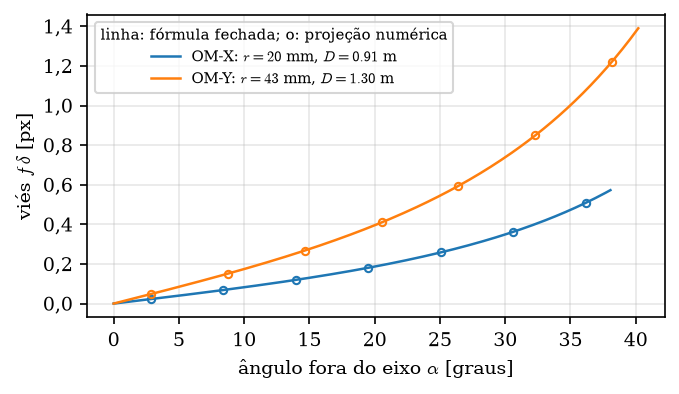
\includegraphics[width=0.62\linewidth]{figuras/vies_perspectiva.png}
\caption{Viés de perspectiva $f\delta$ (Eq.~\ref{eq:bias}) entre o centro da
silhueta e a projeção do centro da esfera, na distância da pose padrão. Os
círculos são a verificação numérica independente.}
\label{fig:bias}
\end{figure}

\begin{proposicao}[MEC sob oclusão]
\label{prop:oclusao}
Seja $\mathcal D$ o disco da silhueta (raio $R$, centro $\vect c$) e
$S\subseteq\mathcal D$ a parte visível, compacta.
\begin{enumerate}
\item[(i)] Se $S$ contém dois pontos antípodas de $\partial\mathcal D$ (por
exemplo, um arco de borda com ângulo $\geq\pi$), então
$\MEC(S)=\mathcal D$ e o centro estimado é exato.
\item[(ii)] Se o oclusor é um semiplano e a parte visível é menor que meio
disco, $S=\mathcal D\cap\{\vect x:\langle\vect x-\vect c,\vect n\rangle\leq-h\}$
com $0<h<R$ e $\|\vect n\|=1$, então $\MEC(S)$ é o disco que tem a corda como
diâmetro: centro $\vect c-h\vect n$, raio $\sqrt{R^2-h^2}$. O erro de centro é
$h$, com fração visível
$f(h)=\bigl[\arccos(h/R)-(h/R)\sqrt{1-h^2/R^2}\bigr]/\pi$.
\end{enumerate}
\end{proposicao}
\begin{proof}
(i) Todo disco que contém dois pontos à distância $2R$ tem raio $\geq R$, e
$\mathcal D\supseteq S$ tem raio $R$. Pela unicidade, $\MEC(S)=\mathcal D$.
(ii) Escreva $\vect x\in S$ como $\vect x=\vect c-s\vect n+w\vect\tau$, com
$\vect\tau\perp\vect n$, $s\geq h$ e $s^2+w^2\leq R^2$. Então
$\|\vect x-(\vect c-h\vect n)\|^2=(s-h)^2+w^2\leq(s-h)^2+R^2-s^2=R^2-h^2-2h(s-h)\leq
R^2-h^2$. Logo, o disco proposto contém $S$. As extremidades da corda,
$s=h$ e $w=\pm\sqrt{R^2-h^2}$, são antípodas nele, e o argumento de (i) conclui.
\end{proof}

A Proposição~\ref{prop:oclusao} mostra a vantagem do MEC sobre o centróide
(momentos de ordem 1). Com até metade do disco oculta por uma borda reta, o MEC
continua exato, enquanto o centróide de meio disco já erra $4R/(3\pi)\approx
0{,}42R$. A Figura~\ref{fig:circ}(b) compara os dois para um disco digital de
$R=30$\,px. No regime~(i), o erro medido do MEC fica $\leq\num{\CircMecErrAboveHalfMax}R$.
O desvio residual em relação à teoria vem do condicionamento: perto da corda
mais larga, a distância aos pontos extremos varia só em segunda ordem com a
posição do centro, e uma perturbação de digitalização $\varepsilon$ desloca o
centro em cerca de $\sqrt{2R\varepsilon}$ (estimativa heurística; para
$\varepsilon\approx0{,}07$\,px, $\approx2$\,px). A circularidade cai
monotonamente com a oclusão (curva traço-ponto). Isso justifica, em parte, usá-la
como confiança.

\begin{figure}[ht]
\centering
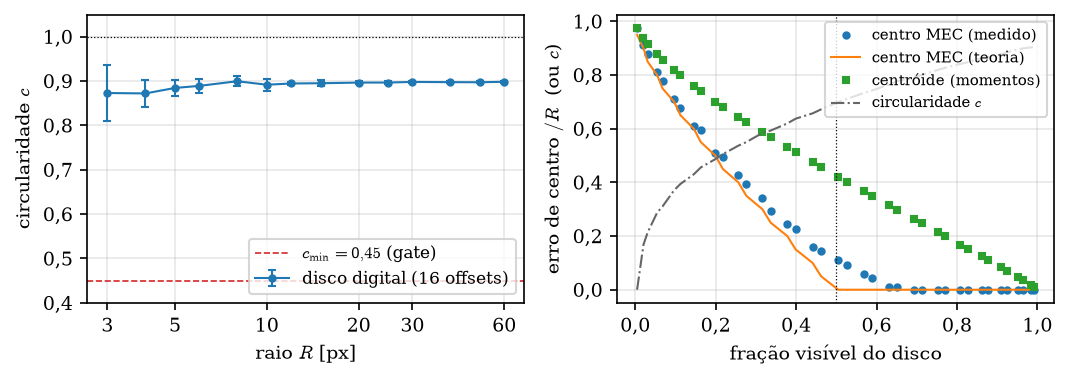
\includegraphics[width=\linewidth]{figuras/circularidade.png}
\caption{(a) Circularidade de discos digitais em função do raio (média e
desvio padrão sobre 16 deslocamentos subpixel); a assíntota é
$c_\infty\approx0{,}899$ (Proposição~\ref{prop:circ-digital}). (b) Oclusão por
semiplano de um disco com $R=30$\,px: erro do centro do MEC (medido e
teórico, Proposição~\ref{prop:oclusao}), erro do centróide e circularidade.}
\label{fig:circ}
\end{figure}

%=====================================================================
\section{Do pixel ao mundo: elevação ao plano da mesa}
\label{sec:elevacao}
%=====================================================================

\subsection{Retroprojeção}

O pixel $(\hat u,\hat v)$ define o raio
\begin{equation}
\vect x(\lambda)=\vect O+\lambda\,\vect d,\qquad
\vect d=R\,K^{-1}\tilde{\vect u}=R\begin{bmatrix}(\hat u-c_x)/f_x\\(\hat v-c_y)/f_y\\1\end{bmatrix},\qquad\lambda>0.
\label{eq:ray}
\end{equation}
O código normaliza $\vect d$ (\code{_pixel_ray_cam}). Isso muda o parâmetro
$\lambda$, mas não o ponto de interseção. Com a forma não normalizada de
\eqref{eq:ray}, como a terceira componente de $K^{-1}\tilde{\vect u}$ é 1,
o valor de $\lambda$ na interseção é igual à profundidade $Z$ do ponto em $\{C\}$.

\subsection{O plano dos centros}

Uma esfera de raio $r$ apoiada num plano horizontal de altura
$z_{\text{mesa}}$ tem o centro em $z=z_{\text{mesa}}+r$. O lifter usa o plano
\begin{equation}
\Pi=\{\vect x\in\R^3:\ \ez\T\vect x=z_\Pi\},\qquad z_\Pi=z_{\text{mesa}}+r,
\end{equation}
com $z_{\text{mesa}}=0$ e $r=\SI{\OmxBallr}{mm}$ (OM-X) ou \SI{\OmyBallr}{mm}
(OMY), lidos de \code{lifter} no YAML. A interseção é
\begin{equation}
\lambda^\star=\frac{z_\Pi-O_z}{d_z},\qquad \hat{\vect p}=\vect O+\lambda^\star\vect d,
\label{eq:lift}
\end{equation}
definida quando $|d_z|\geq10^{-12}$ (raio não paralelo ao plano) e
$\lambda^\star>0$ (plano à frente da câmera). Caso contrário, a vista é
descartada (\code{intersect_ray_horizontal_plane}).

\begin{proposicao}[Exatidão do modelo]
\label{prop:exato}
Se o centro verdadeiro $\vect p^\star$ está em $\Pi$, está à frente da câmera e
$(\hat u,\hat v)=\pi(\vect p^\star)$ é sua projeção exata pela
Eq.~\eqref{eq:proj}, então a Eq.~\eqref{eq:lift} devolve $\hat{\vect p}=\vect p^\star$.
\end{proposicao}
\begin{proof}
Pela definição de projeção central, $\vect p^\star=\vect O+Z^\star\vect d$ com
$\vect d$ dado por \eqref{eq:ray} e $Z^\star>0$. Como $d_z\neq0$, a reta
encontra $\Pi$ em um único ponto, que portanto é $\vect p^\star$.
\end{proof}

Assim, com uma única câmera, o erro de posição vem apenas de três fontes: erro
no pixel do centro (viés da Proposição~\ref{prop:elipse}, oclusão,
digitalização), erro no modelo do plano ($z_\Pi$) e erro de calibração. Essas
fontes são quantificadas na Seção~\ref{sec:erro}. Uma consequência importante
é que a altura estimada é sempre $z_\Pi$ por construção, de modo que o erro em
$z$ é nulo enquanto a bola de fato está sobre a mesa.

\subsection{Fusão de múltiplas vistas}
\label{sec:fusao}

Para cada câmera $i$ configurada que produziu uma detecção, o lifter fica com a
de maior confiança (o detector já retorna no máximo uma), calcula
$\hat{\vect p}_i$ por \eqref{eq:lift} e funde
\begin{equation}
\hat{\vect p}=\sum_i w_i\,\hat{\vect p}_i,\qquad
w_i=\frac{\max(\kappa_i,10^{-3})}{\sum_j\max(\kappa_j,10^{-3})},
\label{eq:fuse}
\end{equation}
e reimpõe $\hat p_z=z_\Pi$ (\code{TablePlanePoseLifter.lift}). Como $\Pi$ é
afim e \eqref{eq:fuse} é uma combinação convexa de pontos de $\Pi$, a
reimposição só remove arredondamento. Basta uma vista: se uma câmera estiver
obstruída, a outra sozinha define $\hat{\vect p}$.

\begin{observacao}[Pesos ótimos]
Se os $\hat{\vect p}_i$ fossem não viesados e independentes, com covariâncias
$\Sigma_i$ no plano, o estimador linear de variância mínima seria
$\hat{\vect p}=(\sum_i\Sigma_i^{-1})^{-1}\sum_i\Sigma_i^{-1}\hat{\vect p}_i$.
A Eq.~\eqref{eq:fuse} usa pesos escalares baseados na circularidade, e não em
$\Sigma_i$. Os dois coincidem quando as vistas têm covariâncias iguais. Sem
oclusão, $\kappa_E\approx\kappa_D\approx0{,}89$ e os pesos ficam
$\approx\frac12$.
\end{observacao}

A saída é um \code{BallObservation} com \code{position_world}$=\hat{\vect p}$,
\code{radius_m}$=r$, \code{timestamp} igual ao maior carimbo de tempo entre os
quadros usados e \code{source} igual ao identificador do pipeline. O campo
\code{covariance} existe no tipo, mas o lifter atual não o preenche
(Seção~\ref{sec:erro} mostra como calculá-lo), e \code{pickable} permanece
\code{None}.

\subsection{Exemplo numérico completo}
\label{sec:exemplo}

A Tabela~\ref{tab:exemplo} acompanha o cálculo na célula OM-X com a bola
na pose de coleta padrão, $\vect p^\star=(\num{\OmxGtX}; \num{\OmxGtY}; \num{\OmxGtZ})$\,mm.
Todos os valores foram obtidos do pipeline real; a reimplementação passo a
passo usada para preencher a tabela reproduz a máscara do detector bit a bit e
a posição fundida com tolerância de $10^{-12}$\,m.

\begin{table}[ht]
\centering
\small
\caption{Exemplo completo, OM-X, pose \code{pick_default}. Comprimentos em
metros, salvo indicação.}
\label{tab:exemplo}
\begin{tabular}{@{}lcc@{}}
\toprule
& câmera esquerda ($E$) & câmera direita ($D$)\\
\midrule
contornos encontrados & \num{\OmxENContours} & \num{\OmxDNContours}\\
área $A$ / perímetro $P$ [px] & \num{\OmxEAreaPx} / \num{\OmxEPerimeterPx} & \num{\OmxDAreaPx} / \num{\OmxDPerimeterPx}\\
circularidade $c=\kappa$ & \num{\OmxECirc} & \num{\OmxDCirc}\\
IoU máscara $\times$ segmentação & \num{\OmxEIou} & \num{\OmxDIou}\\
centro MEC $(\hat u,\hat v)$ [px] & (\num{\OmxEU}; \num{\OmxEV}) & (\num{\OmxDU}; \num{\OmxDV})\\
projeção exata $\pi(\vect p^\star)$ [px] & (\num{\OmxEUGt}; \num{\OmxEVGt}) & (\num{\OmxDUGt}; \num{\OmxDVGt})\\
erro de centro [px] & \num{\OmxECentreErrPx} & \num{\OmxDCentreErrPx}\\
viés previsto $f\delta$ (Eq.~\ref{eq:bias}) [px] & \num{\OmxEEllBias} & \num{\OmxDEllBias}\\
raio MEC $\hat\rho$ / previsto $fa$ [px] & \num{\OmxERadiusPx} / \num{\OmxEEllA} & \num{\OmxDRadiusPx} / \num{\OmxDEllA}\\
\midrule
$K^{-1}\tilde{\vect u}$ & (\num{\OmxEDcX}; \num{\OmxEDcY}; \num{\OmxEDcZ}) & (\num{\OmxDDcX}; \num{\OmxDDcY}; \num{\OmxDDcZ})\\
$\vect d=RK^{-1}\tilde{\vect u}$ & (\num{\OmxEDwX}; \num{\OmxEDwY}; \num{\OmxEDwZ}) & (\num{\OmxDDwX}; \num{\OmxDDwY}; \num{\OmxDDwZ})\\
centro óptico $\vect O$ & (\num{\OmxEOX}; \num{\OmxEOY}; \num{\OmxEOZ}) & (\num{\OmxDOX}; \num{\OmxDOY}; \num{\OmxDOZ})\\
$\lambda^\star=(z_\Pi-O_z)/d_z$ & \num{\OmxET} & \num{\OmxDT}\\
profundidade $Z$ de $\vect p^\star$ & \num{\OmxEDepth} & \num{\OmxDDepth}\\
$\hat{\vect p}_i$ [mm] & (\num{\OmxEPX}; \num{\OmxEPY}; \num{\OmxEPZ}) & (\num{\OmxDPX}; \num{\OmxDPY}; \num{\OmxDPZ})\\
peso $w_i$ & \num{\OmxEWeight} & \num{\OmxDWeight}\\
\midrule
$\hat{\vect p}$ fundido [mm] & \multicolumn{2}{c}{(\num{\OmxFuX}; \num{\OmxFuY}; \num{\OmxFuZ})}\\
erro $\|\hat{\vect p}-\vect p^\star\|_{xy}$ / $|\Delta z|$ [mm] & \multicolumn{2}{c}{\num{\OmxExXyerr} / \num{\OmxExZerr}}\\
\bottomrule
\end{tabular}
\end{table}

Note que $\lambda^\star$ coincide com a profundidade $Z$, como previsto. Na
célula OMY, na pose padrão $(\num{\OmyGtX}; \num{\OmyGtY})$\,mm, o mesmo cálculo
dá $\hat{\vect p}=(\num{\OmyFuX}; \num{\OmyFuY}; \num{\OmyFuZ})$\,mm, com erro
horizontal de \SI{\OmyExXyerr}{mm}. A Figura~\ref{fig:geom} mostra os raios e
os erros no plano.

\begin{figure}[ht]
\centering
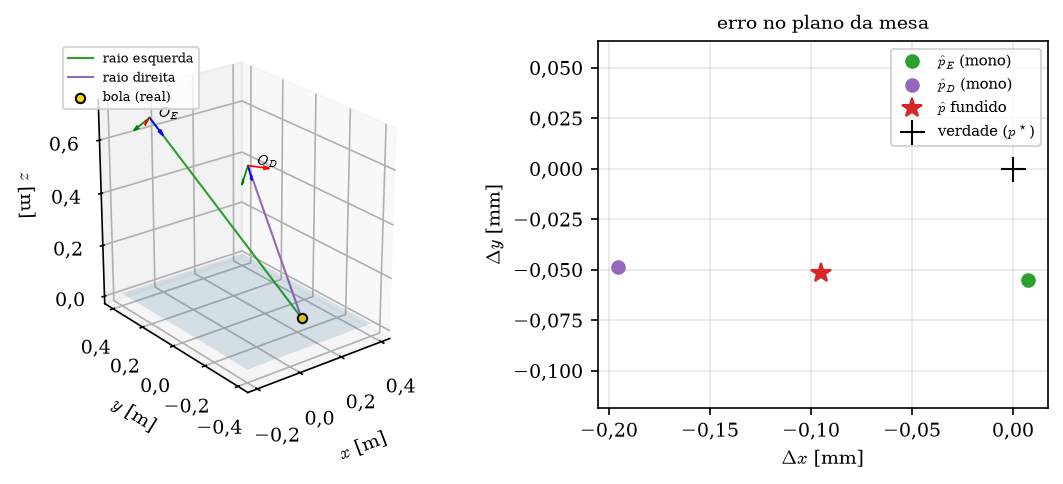
\includegraphics[width=\linewidth]{figuras/geometria_omx.png}
\caption{Esquerda: raios de retroprojeção das duas câmeras (eixos $x_C,y_C,z_C$
em vermelho, verde e azul) até o plano $\Pi$ (OM-X). Direita: erro das
estimativas monoculares e da fundida no plano da mesa, em milímetros.}
\label{fig:geom}
\end{figure}

%=====================================================================
\section{Análise de erro}
\label{sec:erro}
%=====================================================================

\subsection{Jacobiano da elevação}

\begin{proposicao}
\label{prop:jac}
Seja $\vect r_k$ a $k$-ésima coluna de $R$. A derivada do ponto
\eqref{eq:lift} em relação ao pixel é
\begin{equation}
\frac{\partial\hat{\vect p}}{\partial u}=\frac{\lambda^\star}{f_x}\Bigl(\vect r_1-\frac{r_{1z}}{d_z}\vect d\Bigr),\qquad
\frac{\partial\hat{\vect p}}{\partial v}=\frac{\lambda^\star}{f_y}\Bigl(\vect r_2-\frac{r_{2z}}{d_z}\vect d\Bigr),
\label{eq:jac}
\end{equation}
com componente $z$ nula. Definimos $J=[\partial_u\hat{\vect p}\ \ \partial_v\hat{\vect p}]_{xy}\in\R^{2\times2}$.
\end{proposicao}
\begin{proof}
De \eqref{eq:ray}, $\partial\vect d/\partial u=\vect r_1/f_x$. De \eqref{eq:lift},
$\partial\lambda^\star/\partial u=-\lambda^\star(\partial d_z/\partial u)/d_z
=-\lambda^\star r_{1z}/(f_xd_z)$. Pela regra do produto,
$\partial\hat{\vect p}/\partial u=(\partial\lambda^\star/\partial u)\vect d+
\lambda^\star\partial\vect d/\partial u$, que é a primeira expressão. A
componente $z$ é $\frac{\lambda^\star}{f_x}(r_{1z}-r_{1z})=0$. O caso de $v$ é
análogo.
\end{proof}

No exemplo, em mm/px,
\[
J_E=\begin{bmatrix}\num{\OmxEJAa}&\num{\OmxEJAb}\\ \num{\OmxEJBa}&\num{\OmxEJBb}\end{bmatrix},\qquad
J_D=\begin{bmatrix}\num{\OmxDJAa}&\num{\OmxDJAb}\\ \num{\OmxDJBa}&\num{\OmxDJBb}\end{bmatrix},
\]
com valores singulares máximos \num{\OmxEJsig} e \num{\OmxDJsig}\,mm/px. A
fórmula \eqref{eq:jac} concorda com diferenças finitas centradas até
\num{\OmxJacFd}\,m/px. A Figura~\ref{fig:sens} mapeia $\sigma_{\max}(J)$ sobre a
mesa. A sensibilidade cresce com a distância e com a obliquidade do raio, e a
fusão com pesos iguais reduz a covariância.

\begin{figure}[ht]
\centering
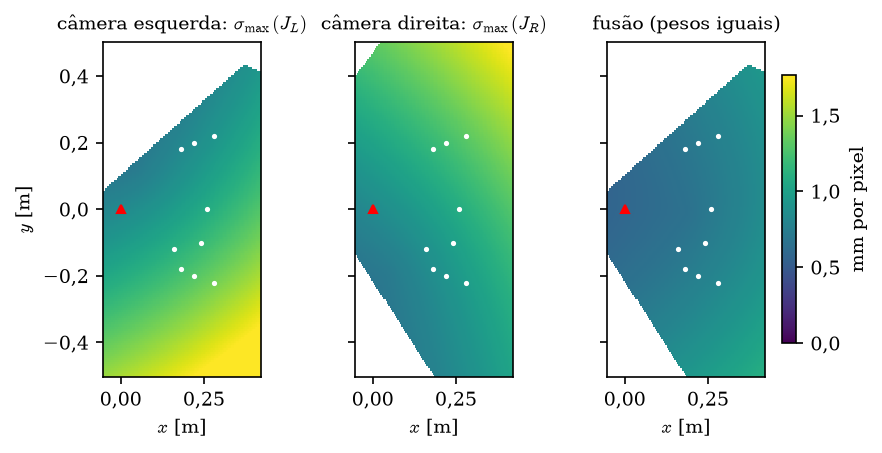
\includegraphics[width=\linewidth]{figuras/sensibilidade_omx.png}\\[2pt]
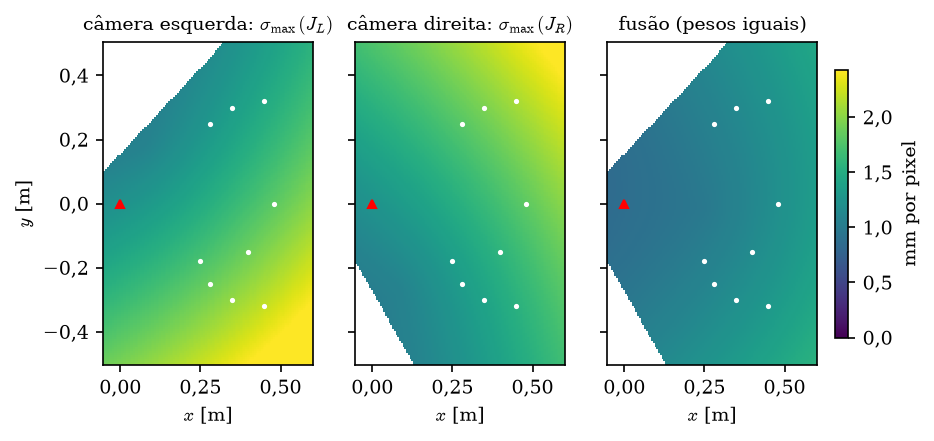
\includegraphics[width=\linewidth]{figuras/sensibilidade_omy.png}
\caption{Sensibilidade $\sigma_{\max}(J)$ do ponto elevado ao erro de pixel
(mm/px) sobre o plano $\Pi$, só onde o ponto projeta dentro da imagem.
Acima: OM-X; abaixo: OMY. Pontos brancos: poses da varredura da
Seção~\ref{sec:resultados}; triângulo: base do braço. O mapa ignora oclusão
pelo robô.}
\label{fig:sens}
\end{figure}

\subsection{Propagação de covariância e verificação de Monte Carlo}

Se o erro do centro em cada vista é independente, com covariância
$\sigma^2I_2$, a linearização dá
\begin{equation}
\Sigma_i\approx\sigma^2J_iJ_i\T,\qquad \Sigma_{\hat{\vect p}}\approx\sum_iw_i^2\,\Sigma_i.
\label{eq:cov}
\end{equation}
Para verificar \eqref{eq:cov}, somamos ruído gaussiano com $\sigma=0{,}5$\,px
aos centros detectados do exemplo, repetimos elevação e fusão
\num{20000} vezes e comparamos a covariância empírica com a prevista. Os
semieixos do elipsoide de $1\sigma$ foram
(\num{\OmxMcEmpMinMm}; \num{\OmxMcEmpMaxMm})\,mm (empírico) e
(\num{\OmxMcPredMinMm}; \num{\OmxMcPredMaxMm})\,mm (previsto), com diferença
relativa de Frobenius de \num{\OmxMcFrobRel} (OMY: (\num{\OmyMcEmpMinMm}; \num{\OmyMcEmpMaxMm}) contra (\num{\OmyMcPredMinMm}; \num{\OmyMcPredMaxMm})\,mm). A
linearização é, portanto, excelente nessa escala, e
\eqref{eq:cov} poderia preencher o campo \code{covariance} do
\code{BallObservation}.

\subsection{Erro no modelo do plano}

Se o centro real está em $z_\Pi+\delta z$ (raio configurado errado, mesa mais
alta ou bola sobre um apoio), o raio que passa pelo centro real encontra $\Pi$
em $\vect p^\star-(\delta z/d_z)\vect d$. O erro horizontal é então
\begin{equation}
\Delta\hat{\vect p}_{xy}=-\delta z\,\frac{\vect d_{xy}}{d_z},\qquad
\|\Delta\hat{\vect p}_{xy}\|=|\delta z|\tan\theta,
\end{equation}
com $\theta$ o ângulo do raio com a vertical. No exemplo, $\tan\theta_E=
\num{\OmxETanIncidence}$ e $\tan\theta_D=\num{\OmxDTanIncidence}$. Na fusão, os
deslocamentos são vetoriais e se cancelam em parte, porque as câmeras estão em
lados opostos: o erro fundido é \num{\OmxDzShift}\,mm por milímetro de $\delta z$
(OMY: \num{\OmyDzShift}). Por exemplo, configurar o raio da bola com
\SI{1}{mm} de erro desloca a estimativa em $\approx\SI{0.6}{mm}$.

\subsection{Erro de calibração}

Uma pequena rotação $\delta\phi$ da câmera desvia todos os raios do mesmo
ângulo, o que equivale, em primeira ordem, a um deslocamento de pixel de
$f\,\delta\phi$. Com $f\approx\num{938}$\,px e $\sigma_{\max}(J)\approx1{,}3$\,mm/px,
\SI{1}{mrad} de erro de orientação vale $\approx\SI{0.94}{px}\approx\SI{1.2}{mm}$.
Um erro de translação $\delta\vect O$ desloca $\hat{\vect p}$ em
$\delta\vect O_{xy}-\delta O_z\,\vect d_{xy}/d_z$. Em simulação, os dois são
nulos até \num{e-10} (Seção~\ref{sec:camera}). Numa célula real, a calibração
extrínseca tende a ser a fonte de erro dominante.

\subsection{Oclusão parcial: estudo de caso}
\label{sec:oclusao-caso}

O caso mais desfavorável da varredura é a pose
\code{mid_backish} do OM-X, com a bola em $(0{,}16;\,-0{,}12)$\,m (Figura~\ref{fig:oclusao}). Na câmera
esquerda, o braço esconde a maior parte da bola: só
\SI{\OccVisibleFrac}{\percent} da silhueta teórica está visível. A circularidade
da parte visível é \num{\OccCirc}, acima de $c_{\min}=0{,}45$, e a detecção é
aceita. O MEC cai no regime~(ii) da Proposição~\ref{prop:oclusao}. Com um
oclusor reto, o modelo preveria $h\approx14$\,px para essa fração visível; o
erro de centro medido é \num{\OccCentreErrPx}\,px (borda do braço não é reta).
A estimativa monocular esquerda erra \SI{\occLeftErr}{mm}, enquanto a direita,
sem oclusão, erra \SI{\occMonoErr}{mm}. Como a circularidade baixa dá peso
$w_E=\num{\occLeftW}$, a fusão atenua, mas não elimina, o erro: o resultado
fundido erra \SI{\occFusedErr}{mm}. Isso ainda fica dentro da tolerância de
\SI{15}{mm} do benchmark, mas mostra o ponto fraco do esquema de pesos
(Seção~\ref{sec:limitacoes}).

\begin{figure}[ht]
\centering
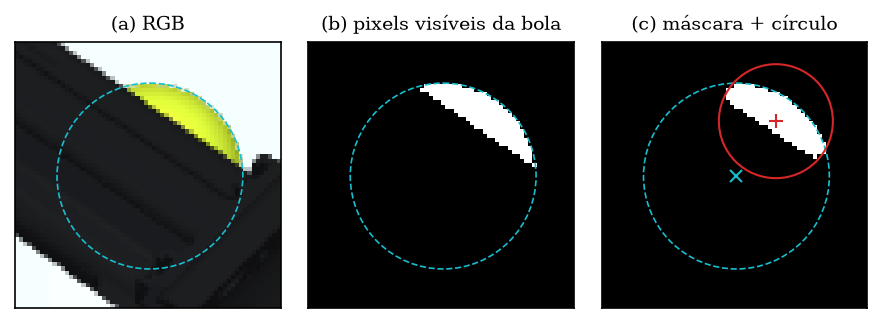
\includegraphics[width=0.78\linewidth]{figuras/oclusao_omx.png}
\caption{Oclusão parcial pelo braço (OM-X, \code{mid_backish}, câmera
esquerda). Tracejado ciano: silhueta teórica completa (Proposição~\ref{prop:elipse});
$\times$: projeção exata do centro; vermelho: MEC da máscara e centro estimado.}
\label{fig:oclusao}
\end{figure}

%=====================================================================
\section{Resultados na simulação}
\label{sec:resultados}
%=====================================================================

As Tabelas~\ref{tab:sweep-omx} e~\ref{tab:sweep-omy} repetem as nove poses de
\code{scripts/benchmark_mujoco_vision.py}. Para cada câmera, a coluna
``visível'' é a razão entre os pixels da bola na segmentação de referência e a
área teórica $\pi f^2ab$ da silhueta. Ela mede diretamente a oclusão.

\begin{table}[ht]
\centering
\footnotesize
\caption{Varredura OM-X ($E$ / $D$ = câmera esquerda / direita). Erro XY da
estimativa fundida em relação à posição real da bola no MuJoCo.}
\label{tab:sweep-omx}
\begin{tabular}{@{}lcccccc@{}}
\toprule
pose & $(x,y)$ [m] & vistas & visível [\%] & $c$ & erro centro [px] & erro XY [mm]\\
\midrule
\tabelagerada{tabela_varredura_omx.tex}
\bottomrule
\end{tabular}
\end{table}

\begin{table}[ht]
\centering
\footnotesize
\caption{Varredura OMY. Em \code{front_cone}, a bola está dentro da caixa de
depósito (paredes de \SI{0.28}{m}); só uma calota de cerca de
\SI{11}{\percent} aparece por cima da parede, e ela não passa nos filtros de
área e circularidade. O pipeline devolve \code{None} e não inventa uma pose.}
\label{tab:sweep-omy}
\begin{tabular}{@{}lcccccc@{}}
\toprule
pose & $(x,y)$ [m] & vistas & visível [\%] & $c$ & erro centro [px] & erro XY [mm]\\
\midrule
\tabelagerada{tabela_varredura_omy.tex}
\bottomrule
\end{tabular}
\end{table}

Para uma visão espacial, a Figura~\ref{fig:mapas} varre a bola numa grade
densa: \num{\OmxGridN} posições no OM-X e \num{\OmyGridN} no OMY, com o braço na
configuração de sensoriamento. Quando as duas câmeras veem mais de
\SI{95}{\percent} da silhueta (\num{\OmxGridClearN} posições no OM-X e
\num{\OmyGridClearN} no OMY), o erro XY tem mediana \SI{\OmxGridClearMedian}{mm}
e máximo \SI{\OmxGridClearMax}{mm} (OM-X), e mediana
\SI{\OmyGridClearMedian}{mm} e máximo \SI{\OmyGridClearMax}{mm} (OMY), de acordo
com a análise de pixel da Seção~\ref{sec:erro}. Nas demais posições, os erros
se concentram em faixas bem definidas: onde o braço ou as paredes da caixa
cobrem parte da bola numa das vistas (regime~(ii) da
Proposição~\ref{prop:oclusao}). Na grade completa, a mediana é
\SI{\OmxGridMedian}{mm} e o percentil 95 é \SI{\OmxGridPjf}{mm} (OM-X); no
OMY, a mediana é \SI{\OmyGridMedian}{mm} e o percentil 95 é
\SI{\OmyGridPjf}{mm}. O OM-X detecta a bola em todas as \num{\OmxGridN}
posições, e o OMY em \num{\OmyGridDet} das \num{\OmyGridN}. As falhas do OMY
ficam dentro da caixa de depósito ou no canto $x\approx0{,}15$\,m,
$y\approx0{,}4$\,m, onde nenhuma câmera vê a bola sem obstrução.

\begin{figure}[ht]
\centering
\begin{subfigure}{0.49\linewidth}
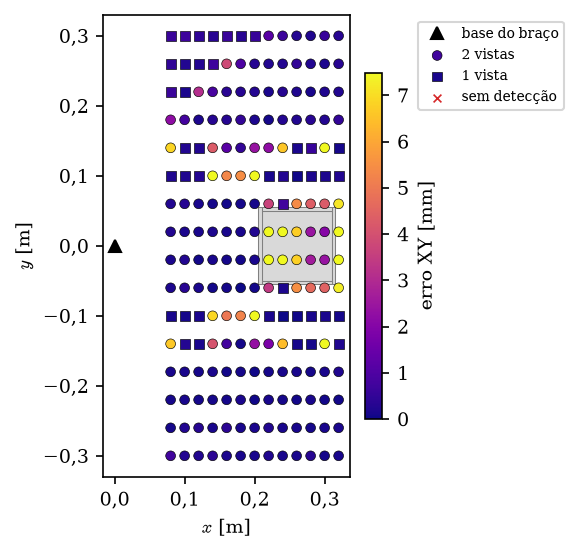
\includegraphics[width=\linewidth]{figuras/mapa_erro_omx.png}
\caption{OM-X}
\end{subfigure}\hfill
\begin{subfigure}{0.49\linewidth}
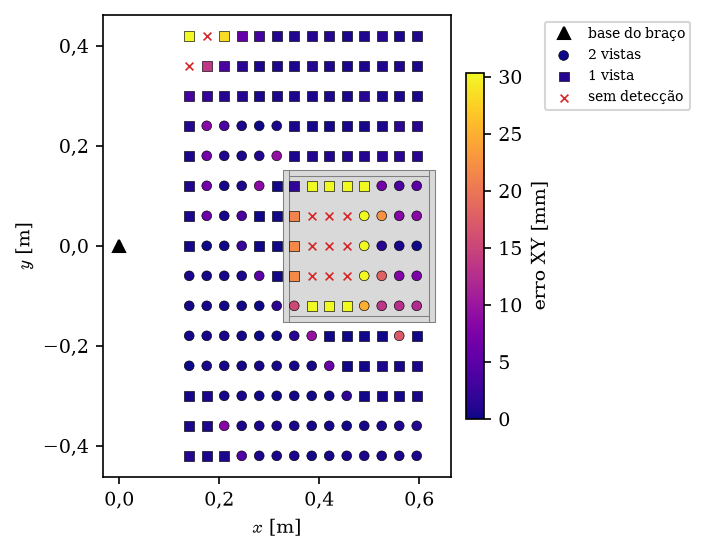
\includegraphics[width=\linewidth]{figuras/mapa_erro_omy.png}
\caption{OMY}
\end{subfigure}
\caption{Erro XY da estimativa fundida numa grade densa de posições da bola.
Círculo: duas vistas; quadrado: uma vista; $\times$: sem detecção. Cinza:
caixa de depósito. A escala de cor satura no percentil 95.}
\label{fig:mapas}
\end{figure}

%=====================================================================
\section{Da posição da bola à pose de preensão}
\label{sec:preensao}
%=====================================================================

\subsection{Por que a posição basta}

Uma esfera homogênea é invariante por qualquer rotação em torno do próprio
centro. A ação de $SE(3)$ sobre a esfera tem estabilizador $SO(3)$ (rotações em
torno do centro), e o espaço de poses distinguíveis é o quociente
$SE(3)/SO(3)\cong\R^3$. Portanto, a ``pose'' do objeto é exatamente a posição
$\hat{\vect p}$ do centro, e é isso que o \code{BallObservation} carrega. A
orientação da garra não é imposta pela visão: ela fica livre e é escolhida pela
cinemática inversa.

\subsection{Alvos cartesianos}

A partir de $\hat{\vect p}$, \code{_pad_mid_pick_waypoints}
(\code{fret/control/pick_place_vision.py}) define três alvos para o ponto médio
entre as pontas dos dedos:
\begin{equation}
\vect p_{\text{hover}}=\hat{\vect p}+h_{\text{hover}}\ez,\qquad
\vect p_{\text{grasp}}=\hat{\vect p}+0{,}012\,\ez,\qquad
\vect p_{\text{lift}}=\hat{\vect p}+h_{\text{lift}}\ez,
\end{equation}
com $(h_{\text{hover}},h_{\text{lift}})=(0{,}08;\,0{,}12)$\,m no OM-X e
$(0{,}10;\,0{,}14)$\,m no OMY. O deslocamento de \SI{12}{mm} acima do centro na
preensão faz os dedos fecharem sobre a esfera sem tocar a mesa. A abertura da
garra é fixada por alvo: aberta em \emph{hover} e fechada (``pinça'') em
\emph{grasp} e \emph{lift}.

\subsection{Cinemática inversa do ponto médio dos dedos}

Seja $\vect m(\vect q)=\frac12\bigl(\vect x_{\text{R}}(\vect q)+\vect x_{\text{L}}(\vect q)\bigr)$
o ponto médio dos centros das geometrias \code{pad_right} e
\code{pad_left}, calculado pela cinemática direta do MuJoCo, com
$\vect q\in\R^n$ ($n=4$ no OM-X e $n=6$ no OMY). Para cada alvo
$\vect p_\ast$, resolve-se
\begin{equation}
\vect q_\ast=\argmin_{\vect q\in[\vect q_{\min},\vect q_{\max}]}\ \|\vect m(\vect q)-\vect p_\ast\|^2
\label{eq:ik}
\end{equation}
pelo método L-BFGS-B \cite{byrd1995} (\code{pad_mid_ik},
\code{fret/control/omy_pad_mid_ik.py}), a partir de várias sementes: a solução
do alvo anterior (\emph{warm start}), as configurações do YAML do cenário e
sementes específicas do robô. Fica a solução de menor resíduo. Se o resíduo
$\|\vect m(\vect q_\ast)-\vect p_\ast\|$ passar de \SI{8}{mm}, a rotina levanta
erro em vez de enviar uma preensão ruim. Como o OM-X tem 4 graus de liberdade e
o alvo tem 3 dimensões, \eqref{eq:ik} tem em geral uma família de soluções; a
escolha entre elas vem das sementes. No exemplo da Tabela~\ref{tab:exemplo},
os resíduos foram \SI{\OmxIkHoverMm}{mm} (\emph{hover}),
\SI{\OmxIkGraspMm}{mm} (\emph{grasp}) e \SI{\OmxIkLiftMm}{mm} (\emph{lift}) no
OM-X, e $\leq\SI{\OmyIkGraspMm}{mm}$ no OMY. Portanto, o erro de posicionamento
cartesiano é dominado pela visão, não pela IK.

\subsection{Integração com a máquina de estados}

Nos simuladores (\code{simulate_pick_place} e
\code{simulate_omy_pick_place}), a visão é chamada uma vez, antes de o braço
dobrar para a postura de repouso. A ordem importa porque a postura dobrada
oclui uma das câmeras. \code{apply_vision_pick_goals}
renderiza as câmeras, executa o pipeline e, se não houver
\code{BallObservation}, levanta erro: o sistema não pega às cegas. Com a
observação, a função substitui as configurações de coleta da máquina de
estados (as de depósito continuam vindo do YAML, pois o depósito é um
\emph{fixture} conhecido) e posiciona a esfera visual \code{cv_ball_ghost} em
$\hat{\vect p}$ (Figura~\ref{fig:overview}).

%=====================================================================
\section{Limitações e melhorias possíveis}
\label{sec:limitacoes}
%=====================================================================

\begin{enumerate}
\item \textbf{Associação entre vistas.} Cada câmera escolhe seu próprio
\emph{blob} de maior circularidade, e nada verifica se as vistas viram o mesmo
objeto. Com duas bolas visíveis, a Eq.~\eqref{eq:fuse} pode fazer a média de
dois objetos diferentes e produzir um ponto entre eles. Um teste de
consistência $\|\hat{\vect p}_E-\hat{\vect p}_D\|\leq\tau$ (por exemplo,
$\tau=3\sqrt{\operatorname{tr}(\Sigma_E+\Sigma_D)}$) resolveria esse caso.
\item \textbf{Oclusão parcial.} A circularidade só reduz o peso de uma vista
oclusa (Seção~\ref{sec:oclusao-caso}). Algumas alternativas: rejeitar vistas
com $\hat\rho$ muito menor que o raio previsto $f\,a(\hat{\vect p})$ (o
Corolário~\ref{cor:mec-elipse} dá a previsão a partir da estimativa da outra
vista), usar pesos de variância mínima com $\Sigma_i$ inflada por $1/c_i$, ou
aplicar o mesmo teste de consistência do item anterior.
\item \textbf{Viés de perspectiva.} É de no máximo $\approx\SI{1.4}{px}$ e
pode ser corrigido de forma fechada pela Eq.~\eqref{eq:bias}.
\item \textbf{Hipótese do plano.} A estimativa de $z$ é imposta. Uma bola
fora da mesa (sobre um obstáculo ou em movimento no ar) gera erro horizontal
de $\delta z\tan\theta$. Com duas vistas, uma triangulação por mínimos
quadrados poderia estimar $z$ e servir de diagnóstico.
\item \textbf{Cor e iluminação.} O limiar HSV é fixo. Funciona bem na
simulação (Figura~\ref{fig:hsv}), mas com câmeras reais precisa de calibração
de cor ou de um modelo de distorção de lente, ausente hoje.
\item \textbf{Incerteza.} O campo \code{covariance} pode ser preenchido com a
Eq.~\eqref{eq:cov}, validada pelo experimento de Monte Carlo.
\end{enumerate}

%=====================================================================
\appendix
\section{Parâmetros das configurações}
%=====================================================================

\begin{table}[H]
\centering
\small
\begin{tabular}{@{}lll@{}}
\toprule
parâmetro & OM-X (\code{omx_portal_overhead.yml}) & OMY (\code{omy_portal_overhead.yml})\\
\midrule
resolução & $1280\times720$ & $1280\times720$\\
\code{fovy} / $f$ [px] & \ang{\OmxFovy} / \num{\OmxFx} & \ang{\OmyFovy} / \num{\OmyFx}\\
centros ópticos $\vect O$ [m] & $(-0{,}12;\ \pm0{,}30;\ 0{,}70)$ & $(-0{,}18;\ \pm0{,}42;\ 0{,}98)$\\
$\vect\ell$ / $\vect h$ (HSV) & $(20;40;40)$ / $(50;255;255)$ & $(20;40;40)$ / $(50;255;255)$\\
elemento estruturante & elíptico $5\times5$ & elíptico $5\times5$\\
$A_{\min}$ / $A_{\max}$ [px$^2$] & 80 / \num{500000} & 120 / \num{500000}\\
$c_{\min}$ & 0,45 & 0,45\\
$z_{\text{mesa}}$ / $r$ [m] & 0 / 0,020 & 0 / 0,043\\
\bottomrule
\end{tabular}
\caption{Parâmetros do pipeline nas duas células com pórtico. Em
\code{config/vision/} também há \code{hsv_blob_overhead.yml} (fixture
sintético, $640\times480$, $c_{\min}=0{,}55$) e
\code{hsv_blob_tennis_yellow.yml} (fotos da web).}
\end{table}

\section{Reprodutibilidade}

Todas as figuras, tabelas e números deste documento são gerados por
\begin{verbatim}
MUJOCO_GL=egl PYOPENGL_PLATFORM=egl python3 scripts/vision_algorithm_figures.py
cd docs/vision/algoritmo-visao && latexmk -pdf algoritmo_visao.tex
\end{verbatim}
O script usa o pipeline de produção (\code{pipeline_from_hsv_plane_config}) e
verifica por asserção que a reimplementação passo a passo coincide com ele:
máscara idêntica, mesmo centro de detecção e posição fundida igual até
$10^{-12}$\,m. As métricas brutas ficam em \code{metricas.json}.

\begin{thebibliography}{9}
\bibitem{hartley2004} R.~Hartley e A.~Zisserman. \emph{Multiple View Geometry in
Computer Vision}, 2.\,ed. Cambridge University Press, 2004.
\bibitem{serra1982} J.~Serra. \emph{Image Analysis and Mathematical Morphology}.
Academic Press, 1982.
\bibitem{suzuki1985} S.~Suzuki e K.~Abe. Topological structural analysis of
digitized binary images by border following. \emph{Computer Vision, Graphics,
and Image Processing}, 30(1):32--46, 1985.
\bibitem{welzl1991} E.~Welzl. Smallest enclosing disks (balls and ellipsoids).
In \emph{New Results and New Trends in Computer Science}, LNCS 555, p.~359--370.
Springer, 1991.
\bibitem{smith1978} A.~R.~Smith. Color gamut transform pairs. \emph{ACM SIGGRAPH
Computer Graphics}, 12(3):12--19, 1978.
\bibitem{freeman1961} H.~Freeman. On the encoding of arbitrary geometric
configurations. \emph{IRE Trans. Electronic Computers}, EC-10(2):260--268, 1961.
\bibitem{byrd1995} R.~H.~Byrd, P.~Lu, J.~Nocedal e C.~Zhu. A limited memory
algorithm for bound constrained optimization. \emph{SIAM J. Sci. Comput.},
16(5):1190--1208, 1995.
\bibitem{opencv} G.~Bradski. The OpenCV Library. \emph{Dr.\ Dobb's Journal of
Software Tools}, 2000.
\end{thebibliography}

\end{document}
